\documentclass{article}

\usepackage{graphicx}
\usepackage{tikz}
\usepackage{tikzsymbols}
\usetikzlibrary{calc,patterns,shapes.geometric}
\pagestyle{empty}
\usepackage[margin=0pt]{geometry}
\geometry{papersize={14in,12in}}

\def\centerarc[#1](#2)(#3:#4:#5){\draw[#1] ($(#2)+({#5*cos(#3)},{#5*sin(#3)})$) arc (#3:#4:#5);}

\begin{document}
	\begin{figure}
		\centering
		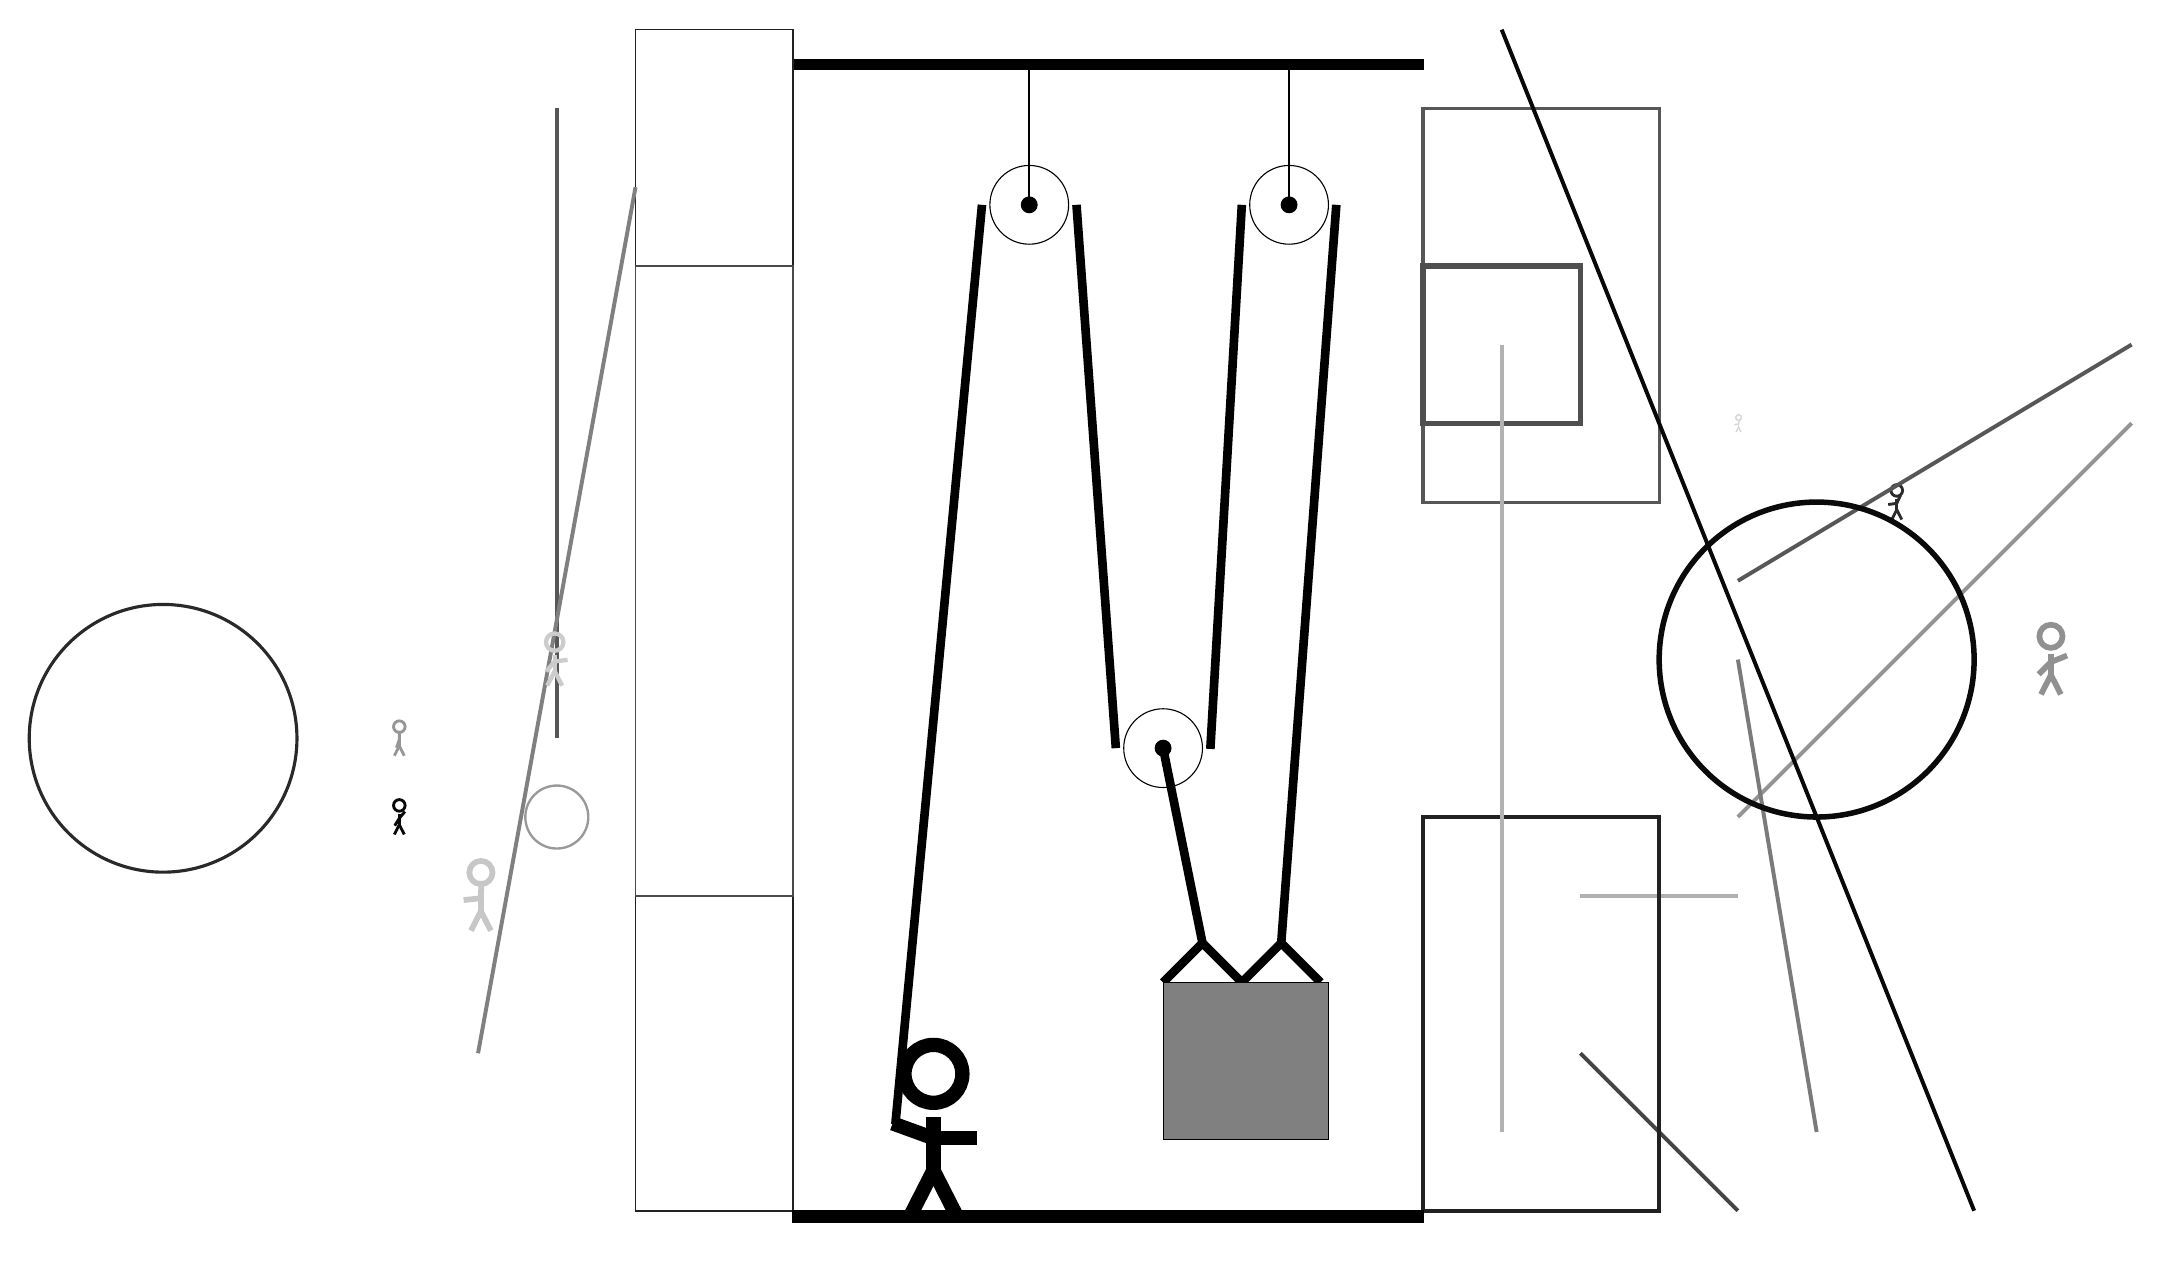
\begin{tikzpicture}
			%%%%% START %%%%%
			
			\draw[fill=black] (-2, 11.5) rectangle (6, 11.625);
			
			\draw (1, 9.775) circle (0.5);
			\draw[fill=black] (1, 9.775) circle (0.1);
			\draw[thick] (1, 9.775) -- (1, 11.5);
			
			\draw[line width=0.4mm, color=black!66] (6, 6) rectangle (9, 11);
			
			\draw[line width=0.4mm, color=black!15] (7, -2) rectangle (7, 2);
			\draw[line width=0.2mm, color=black!87] (-2, -3) rectangle (-4, 12);
			\draw[line width=0.5mm, color=black!31](10, 1) -- (8, 1);
			\draw [line width=0.3mm, color=black!40](-5, 2) circle (0.4);
			\node[line width=0.2mm, color=black!16] at (10, 7) {\Strichmaxerl[1][10][80]};
			\draw[line width=0.5mm, color=black!73](8, -1) -- (10, -3);
			\draw[line width=0.5mm, color=black!42](10, 2) -- (15, 7);
			\draw[line width=0.2mm, color=black!71] (-2, 9) rectangle (-4, 1);
			
			\node[line width=0.5mm, color=black!43] at (14, 4) {\Strichmaxerl[4][45][22]};
			\node[line width=0.3mm, color=black!83] at (12, 6) {\Strichmaxerl[2][8][65]};
			
			\draw[line width=0.7mm, color=black!69] (8, 9) rectangle (6, 7);
			\draw[line width=0.5mm, color=black!52](11, -2) -- (10, 4);
			\node[line width=0.3mm, color=black!97] at (-7, 2) {\Strichmaxerl[2][58][50]};
			\draw [line width=0.7mm, color=black!38](7, 2) circle (0.0);
			\draw [line width=0.4mm, color=black!84](-10, 3) circle (1.7);
			\draw[line width=0.5mm, color=black!87] (6, 2) rectangle (9, -3);
			\node[line width=0.3mm, color=black!22] at (-6, 1) {\Strichmaxerl[4][6][88]};
			\draw[line width=0.5mm, color=black!66](10, 5) -- (15, 8);
			\draw[line width=0.5mm, color=black!30](7, -2) -- (7, 8);
			\draw[line width=0.5mm, color=black!66](-5, 3) -- (-5, 11);
			
			\draw[line width=0.5mm, color=black!50](-4, 10) -- (-6, -1);
			
			\node[line width=0.3mm, color=black!41] at (-7, 3) {\Strichmaxerl[2][71][89]};
			\node[line width=0.7mm, color=black!20] at (-5, 4) {\Strichmaxerl[3][50][7]};
			\draw[line width=0.5mm, color=black!97](7, 12) -- (13, -3);
			\draw [line width=0.7mm, color=black!96](11, 4) circle (2.0);
			
			\draw (4.3, 9.775) circle (0.5);
			\draw[fill=black] (4.3, 9.775) circle (0.1);
			\draw[thick] (4.3, 9.775) -- (4.3, 11.5);
			
			\draw (2.7, 2.875) circle (0.5);
			\draw[fill=black] (2.7, 2.875) circle (0.1);
			
			\draw[line width=1.1mm]  (2.7, -0.1) -- (3.2, 0.4) -- (3.7, -0.1) -- (4.2, 0.4) -- (4.7, -0.1);
			\draw[fill=black!50] (2.7, -0.1) rectangle (4.8, -2.1);
			
			\draw[line width=1.1mm](-0.7, -1.9) -- (0.4, 9.775);
			\centerarc[line width=1.1mm](1, 9.775)(0:180:0.6);
			\draw[line width=1.1mm](1.6, 9.775) -- (2.1, 2.875);
			\centerarc[line width=1.1mm](2.7, 2.875)(180:370:0.6);
			\draw[line width=1.1mm] (3.3, 2.865) -- (3.7, 9.775);
			\centerarc[line width=1.1mm](4.3, 9.775)(0:180:0.6);
			\draw[line width=1.1mm](4.2, 0.4) -- (4.9, 9.775);
			\draw[line width=1.1mm] (3.2, 0.4) -- (2.7, 2.875);
			
			\node at (-0.2, -2) {\Strichmaxerl[10][-20][0]};
			
			\draw[fill=black] (-2, -3) rectangle (6, -3.15);
			
			%%%%% END %%%%%
		\end{tikzpicture}
	\end{figure}	
\end{document}